\subsection{Enunciado del Problema:}

Implemente un scheduler Round-Robin que no permita la migración de procesos entre núcleos (SchedRR2). La asignación de CPU se debe realizar en el momento en que se produce la carga de un proceso (load). El nucleo correspondiente a un nuevo proceso sera aquel con menor cantidad de procesos activos totales (RUNNING + BLOCKED + READY). Disene y realice un conjunto de experimentos que permita evaluar comparativamente las dos implementaciones de Round-Robin.

\subsection{Explicación de la implementacion}

Para implementar esta política de scheduling utilizamos las siguientes estructuras:
\begin{itemize}
	\item Un vector para almacenar el valor del quantum de cada núcleo del procesador.
	\item Un vector que contiene la cola de procesos \textit{ready} de cada núcleo.
	\item Un vector que almacena cuantos procesos bloqueados hay en cada núcleo.
	\item Un diccionario que indica a que núcleo esta asignado cada proceso.
\end{itemize}

Cada vez que un proceso se añade al scheduler calculamos, para cada núcleo, la cantidad de procesos activos, es decir: $RUNNING\ +\ BLOCKED\ +\ READY$. El núcleo con tenga el menor valor en dicha suma sera el núcleo asignado al nuevo proceso.
Entonces, en el diccionario añadimos una entrada para la clave del \textit{pid} del proceso y como valor colocamos el núcleo elegido. De esta forma siempre sabemos a que núcleo fue asignado el proceso.

Cuando un proceso se bloquea, incrementamos en uno el contador de procesos bloqueados del núcleo en el que el proceso se ejecuto. Cuando se desbloquea, lo disminuimos en uno y colocamos el proceso en la cola de procesos \textit{ready} del núcleo que se le asigno al ser cargado.

Cuando debemos determinar el próximo proceso a ejecutar en un núcleo, simplemente tomamos el primer elemento de la cola de procesos \textit{ready} correspondiente a dicho núcleo.

\subsection{Comparación entre los algoritmos de Round Robin}

En todas las pruebas subsecuentes utilizamos la siguiente configuración del simulador:
\begin{itemize}
	\item \textbf{Dos (2) núcleos}. Ya que con un solo núcleo los algoritmos se comportarían exactamente igual y con dos núcleos ya es posible mostrar las diferencias en el comportamiento.
	\item \textbf{Costo de cambio de contexto}: Un (1) ciclo de reloj.
	\item \textbf{Costo de migración de núcleo}: Dos (2) ciclos de reloj.
	\item \textbf{Quantum de cada núcleo}: Dos (2) ciclos de reloj.
\end{itemize}

\subsubsection{Primer experimento}

En este primer experimento solo ejecutamos tareas que utilizan intensivamente el CPU durante diferente tiempo. El lote utilizado es el siguiente:

\begin{quote}
@1\\
TaskCPU 15\\
@3\\
TaskCPU 5\\
TaskCPU 15\\
@4\\
TaskCPU 2
\end{quote}

El resultado de utilizar RR y RR2 fue:

\begin{figure}[H]
\begin{center}
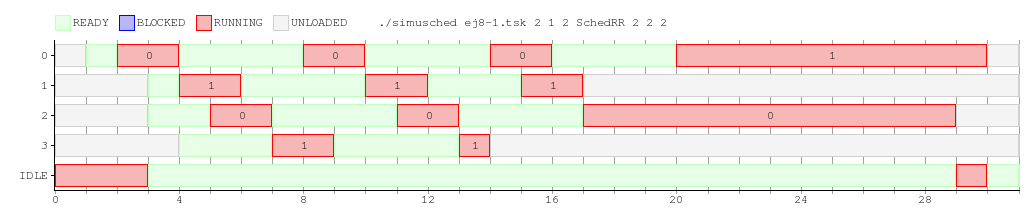
\includegraphics[width=1.1\textwidth]{img/ej8-1-RR.png}
     \caption{Round Robin con migración entre núcleos}
\end{center}
\end{figure}

\begin{figure}[H]
\begin{center}
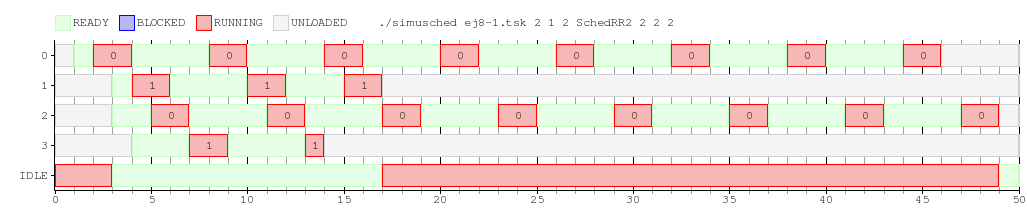
\includegraphics[width=1.1\textwidth]{img/ej8-1-RR2.png}
     \caption{Round Robin sin migración entre núcleos}
\end{center}
\end{figure}

Como se puede observar en los gráficos, la migración entre núcleos permite al primer scheduling terminar mucho mas rápido \textit{(20 ciclos antes, aunque esta diferencia podría ser arbitrariamente grande)} que el segundo, que no permite migrar procesos entre núcleos.
Esto se debe a que, en el segundo scheduler, se asigna el núcleo cero a las dos tareas mas largas \textit{(tareas 0 y 2)}. Entonces, al no estar permitida la migración entre núcleos, el núcleo cero debe ejecutar ambas tareas mientras el núcleo uno esta ocioso \textit{(lo cual es algo totalmente indeseado)}.

\subsubsection{Segundo experimento}

En el segundo experimento utilizamos tareas que utilizan intensivamente la E/S.
El lote utilizado fue el siguiente:

\begin{quote}
@1\\
TaskConsola 6 3 3\\
@3\\
TaskConsola 5 5 5\\
TaskConsola 4 7 7\\
@4\\
TaskConsola 6 4 4\\
\end{quote}

El resultado de utilizar RR y RR2 fue:

\begin{figure}[H]
\begin{center}
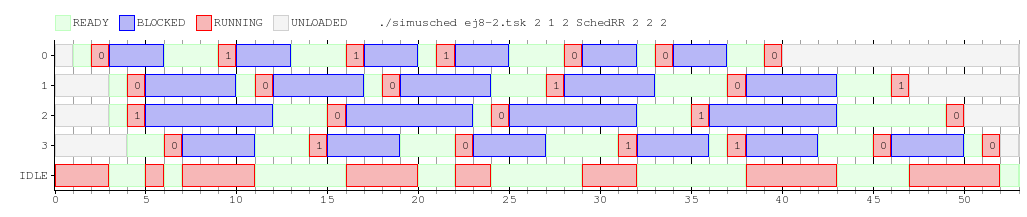
\includegraphics[width=1.1\textwidth]{img/ej8-2-RR.png}
     \caption{Round Robin con migración entre núcleos}
\end{center}
\end{figure}

\begin{figure}[H]
\begin{center}
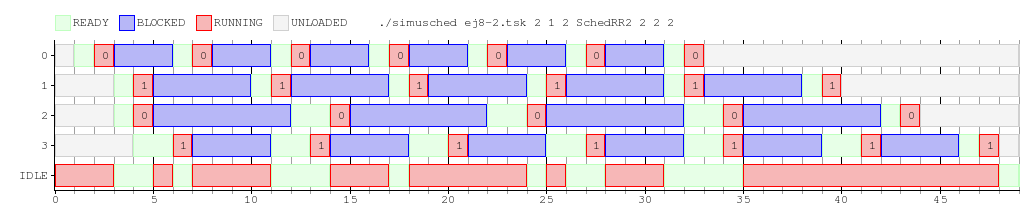
\includegraphics[width=1.1\textwidth]{img/ej8-2-RR2.png}
     \caption{Round Robin sin migración entre núcleos}
\end{center}
\end{figure}

Como se puede ver en los gráficos, en este caso el scheduler Round Robin que no permite la migración entre núcleos termina antes que el si lo permite. Esto es debido a que el costo de migrar un proceso de un núcleo a otro es mayor que el costo que tendría esperar a que el núcleo que se le asigno previamente quede libre, pues las tareas se bloquean muy rápidamente.

\subsubsection{Conclusión}

En algunos casos, puede resultar beneficioso que un proceso espere al núcleo que tenia asignado previamente antes que realizar un migración. Pero, si dicho núcleo no se libera rápidamente y, ademas, teníamos otro núcleo libre, hubiera sido mejor pagar el costo de una migración entre núcleos.

En el primer experimento solo teníamos una tarea a la espera de que su núcleo asignado se libere, mientras había otro núcleo libre. Pero, fácilmente, podría generarse un escenario donde la cantidad de procesos a la espera de un núcleo sea arbitrariamente grande y que la cantidad de núcleos libres también sea arbitrariamente grande, dando como resultado una asignación muy ineficiente de los recursos disponibles.

Por lo dicho, podemos concluir que permitir la migración entre núcleos es, en la mayoría de los casos, mas conveniente que prohibirlo.
